\begin{figure}[H]
  \centering
  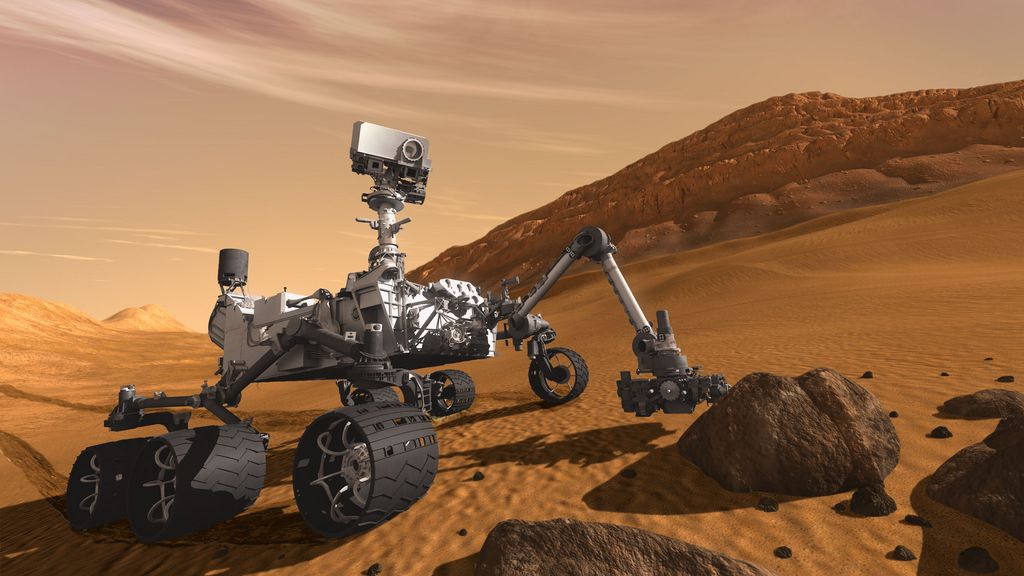
\includegraphics[scale=0.5]{fig/marsRover.jpg}
  \caption{Curiosity Rover with an embedded camera on a arm \cite{nasa}}
  \label{fig:CuriosityRover}
\end{figure}

In this report, we assume that we would like to send a rover on Mars, capable of communicating with Earth. Self-powered by solar panels, it will land at latitude 50� where it could get enough sunlight to recharge its lithium batteries. It is provided with an arm whose hand is replaced with a camera (see figure \ref{fig:CuriosityRover}). The latter will be used by scientists to observe relevant rocks to study. In order to accomplish this mission, once a stone is designed, the camera must be able to keep it in focus, despite the wind, the movement of the robot or any other perturbation. This implies a real time image analysis to be able to rectify the position of the camera. As a robust method is needed to maintain the stone in front of the arm, the correspondence problem is achieved by carrying out a 3D map of the surface. A luminous source should then be added to the rover to be projected on the surface containing the rock and detected by the camera.

This luminous source must be powerful enough to outshine the sunlight during the day, notwithstanding that the energy needed to make it work has to be negligible compared to the amount provided to the rover. Moreover, the characteristics of the camera need to be perfectly adapted to Mars, as once the rover has landed on the red planet, it would be impossible to adjust it. 

Will it be feasible to design such an embedded system, composed of a camera, a luminous source and algorithms, capable of keeping a rock in focus thanks to a 3D map, for an application on Mars soil? 
